%%%%%%%%%%%%%%%%%%%%%%%%%%%%%%%%%%%%%%%%%
% Imperial College London Presentation
% LaTeX Template
% Version 1.0 (April 16, 2024)
%
% This template was created by:
% Vel (enquiries@latextypesetting.com)
% LaTeXTypesetting.com
%
%!TEX program = xelatex
% Note: this template must be compiled with XeLaTeX rather than PDFLaTeX
% due to the custom fonts used. The line above should ensure this happens
% automatically, but if it doesn't, your LaTeX editor should have a simple toggle
% to switch to using XeLaTeX.
%
% © Imperial College London, 2024. This template, including logo and fonts, is 
% for use of Imperial staff and students only for university business. All rights 
% reserved to the copyright owners.
%
%%%%%%%%%%%%%%%%%%%%%%%%%%%%%%%%%%%%%%%%%

%----------------------------------------------------------------------------------------
%	CLASS, PACKAGES AND OTHER DOCUMENT CONFIGURATIONS
%----------------------------------------------------------------------------------------

\documentclass[
	aspectratio=169, % Uncomment to use an aspect ratio of 16:9 (160 mm by 90 mm)
	%aspectratio=43, % Uncomment to use an aspect ratio of 4:3 (128mm by 96mm)
	t, % Top align all slide content by default
	onlytextwidth, % Typeset content in columns at text width
	10pt, % Default font size, use 10pt for the 16:9 aspect ratio and 8pt for the 4:3 aspect ratio
]{beamer}

\usetheme{Imperial} % Use the Imperial theme

%----------------------------------------------------------------------------------------
%	IMPERIAL BEAMER THEME USAGE NOTES
%----------------------------------------------------------------------------------------

% This theme features several predefined Imperial colors which can be used for text and slide backgrounds:
% ICLBlue - Most common slide background color and text color to use (on light backgrounds)
% ICLDarkBlue - Optional darker blue color for slide backgrounds and text
% ICLCream - Accessible background color for use on slide backgrounds
% ICLLightGrey - Accessible background color for use on slide backgrounds

% You can choose to use a 16:9 aspect ratio (default) or a 4:3 aspect ratio by uncommenting the relevant line in the \documentclass specifications above. Note that if you switch between the 2 aspect ratios, you will likely need to adjust how your images are included in the presentation. Usually for a 16:9 aspect ratio, images will be included as width=\paperwidth, but for a 4:3 aspect ratio it's recommended to use height=\paperheight instead.

%----------------------------------------------------------------------------------------
%	PRESENTATION INFORMATION
%----------------------------------------------------------------------------------------

\title{Bayesian Phylolinguistic Inference under
Cognate Dependence} % Presentation title to appear on the title slide and left footers

\subtitle{A Study of Model
Misspecification} % Presentation subtitle to appear on the title slide

\author{Yong Sheng James Tay} % Author name(s) to appear on the title slide

\date{15/06/2026} % Presentation date to appear on the title slide and right footers
\usepackage{multirow}
\usepackage{natbib} 

%----------------------------------------------------------------------------------------

\begin{document}

% \begingroup
% 	\setbeamercolor{background canvas}{bg=ICLLightGrey} % Slide background color
% 	\setbeamercolor{title page title}{fg=ICLBlue} % Title text color
% 	\setbeamercolor{title page subtitle}{fg=ICLBlue} % Subtitle text color
% 	\setbeamercolor{author}{fg=ICLBlue} % Author(s) text color
% 	\setbeamercolor{date}{fg=ICLBlue} % Date text color
% 	\setbeamertemplate{title page}[logo]{ICL_Logo_Blue.pdf} % Imperial logo color, use 'ICL_Logo_White.pdf' for white and 'ICL_Logo_Blue.pdf' for blue
% 	\frame[plain, s]{\titlepage} % Output the title page with no footer ('plain') and vertically distributed text ('s')
% \endgroup

\begin{frame}
	\frametitle{Background}
    Goal: Reconstruct language tree $T^*$ from data $\mathbf{D}$ using Bayesian phylogenetic analysis
\begin{table}[h]
  \centering
  % Left table (Table 1)
  \begin{minipage}{0.55\textwidth}
    \centering
    \begin{tabular}{lcc|cc}
      \toprule
      \multirow{2}{*}{Language} & \multicolumn{2}{c}{\textit{`to laugh'}} & \multicolumn{2}{c}{\textit{`wing'}} \\
      \cmidrule(lr){2-3} \cmidrule(lr){4-5}
      & Word & Class & Word & Class \\
      \midrule
      Fijian & dredre & tl-A & taba-na & w-A \\
      Marquesan & kata & tl-B & peheu & w-B \\
      Hawaiian & 'aka & tl-B & 'heu & w-B \\
      Maori & kata & tl-B & parirau & w-C \\
      Tahitian & 'ata & tl-B & pererau & w-C \\
      \bottomrule
    \end{tabular}
  \end{minipage}
  \hfill
  % Right table (Table 2)
  \begin{minipage}{0.40\textwidth}
    \centering
    \begin{tabular}{l|ccccc}
      \toprule
      \multirow{2}{*}{Language} & \multicolumn{2}{c}{\textit{`to laugh'}} & \multicolumn{3}{c}{\textit{`wing'}} \\
      \cmidrule(lr){2-3} \cmidrule(lr){4-6}
      & A & B & A & B & C \\
      \midrule
      Fijian & 1 & 0 & 1 & 0 & 0 \\
      Marquesan & 0 & 1 & 0 & 1 & 0 \\
      Hawaiian & 0 & 1 & 0 & 1 & 0 \\
      Maori & 0 & 1 & 0 & 0 & 1 \\
      Tahitian & 0 & 1 & 0 & 0 & 1 \\
      \bottomrule
    \end{tabular}
  \end{minipage}
  
  \caption{Binary encoding of cognacy classes from five Oceanic languages. Adapted from Hoffman et al. (2021).}
  \label{tab:cognatedefinition}
\end{table}
    \textbf{Problematic Assumption: Conditional Site Independence}
\end{frame}

% \begin{frame}
% 	\frametitle{Research Questions}
%     \textbf{Question 1} \\ How does unknown site dependence within data hurt tree reconstruction? \\
%     {\color{white} blank}
%     \\
%     \textbf{Question 2} \\ Does adding dependent sites improve tree reconstruction?
%     \\
%     \begin{figure}
%         \centering
%         
\includegraphics[width=1\linewidth]{figures/methods.png}
%         \caption{Factorial Design of experiments.}
%     \end{figure}
% \end{frame}

\begin{frame}
    \frametitle{Results from Experiments}
    \textbf{Experiment 1} (Unknown Dependency Structure)
    \vspace{-3mm}
    \begin{columns}[T]
        \begin{column}{0.48\textwidth}
            \textbf{Small Dataset}
            \vspace{-5mm}
            \begin{figure}
                \centering
                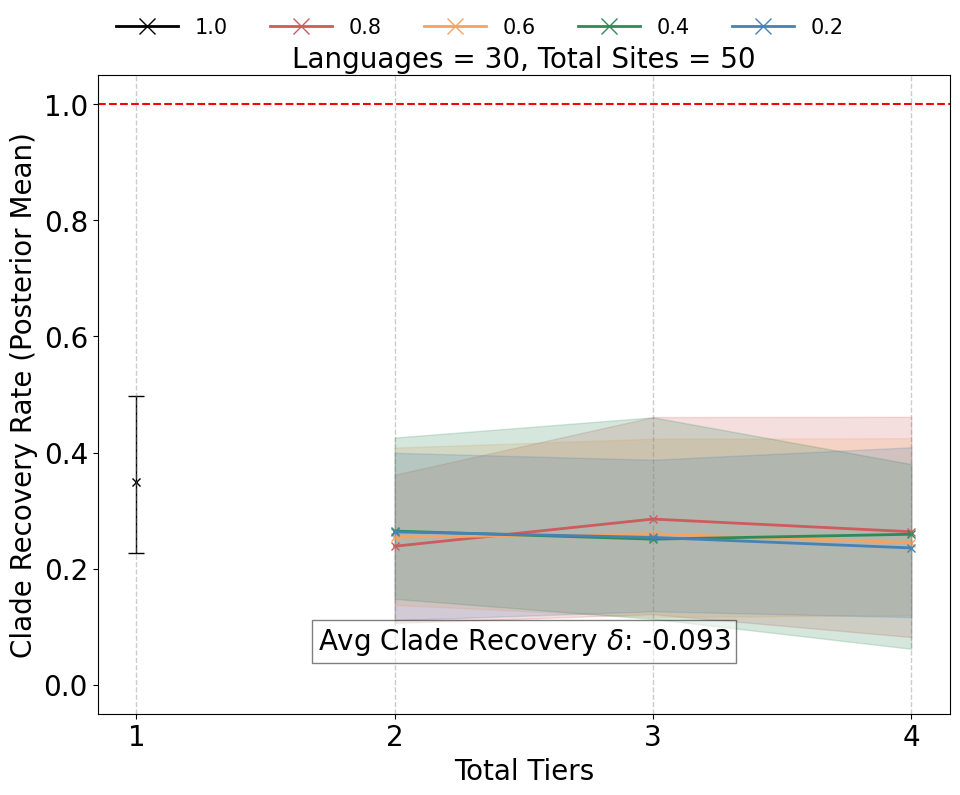
\includegraphics[width=1\linewidth]{figures/exp1lowdata.png}
            \end{figure}
        \end{column}

        \begin{column}{0.48\textwidth}
            \textbf{Large Dataset}
            \vspace{-5mm}
            \begin{figure}
                \centering
                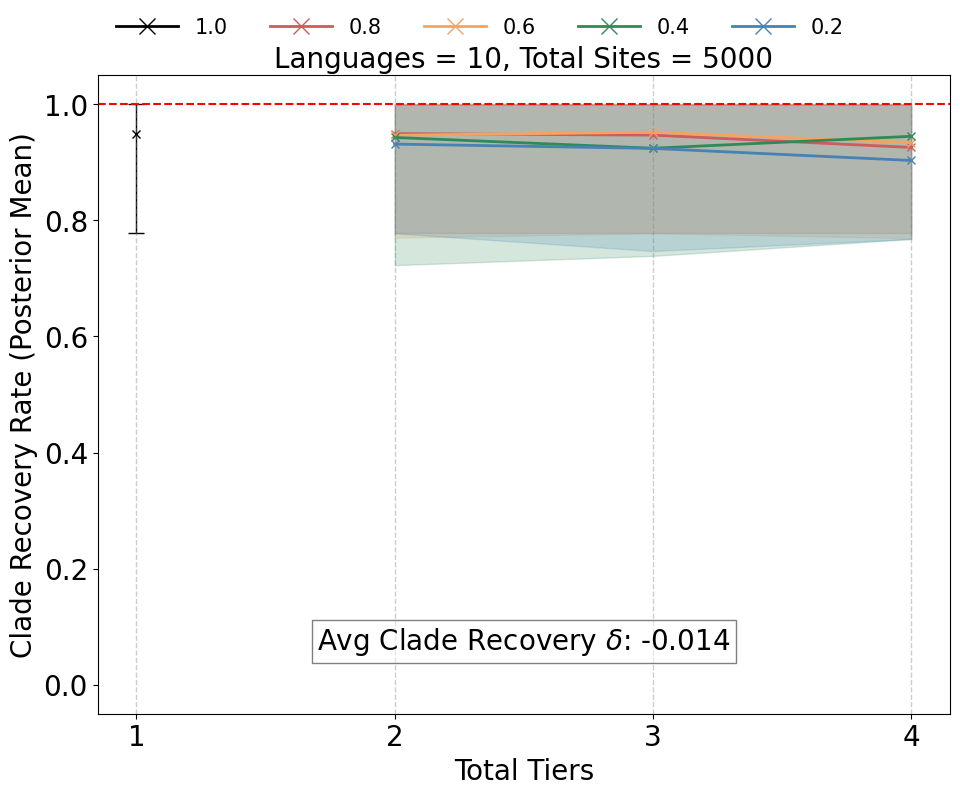
\includegraphics[width=1\linewidth]{figures/exp1highdata.png}
            \end{figure}
        \end{column}
    \end{columns}
\end{frame}

\begin{frame}
    \frametitle{Results from Experiments}
    \textbf{Experiment 2} (Additional Dependent Sites)
    \vspace{-3mm}
    \begin{columns}[T]
        \begin{column}{0.48\textwidth}
            \textbf{Small Dataset}
            \vspace{-5mm}
            \begin{figure}
                \centering
                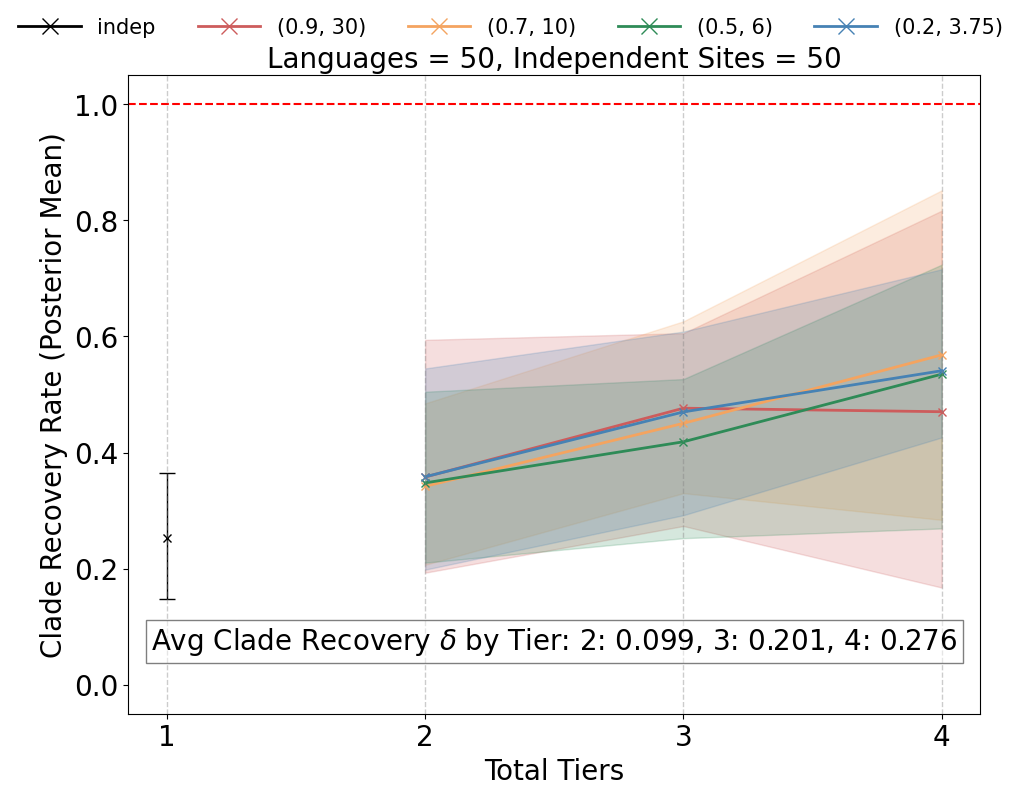
\includegraphics[width=1\linewidth]{figures/exp2lowdata.png}
            \end{figure}
        \end{column}

        \begin{column}{0.48\textwidth}
            \textbf{Large Dataset}
            \vspace{-5mm}
            \begin{figure}
                \centering
                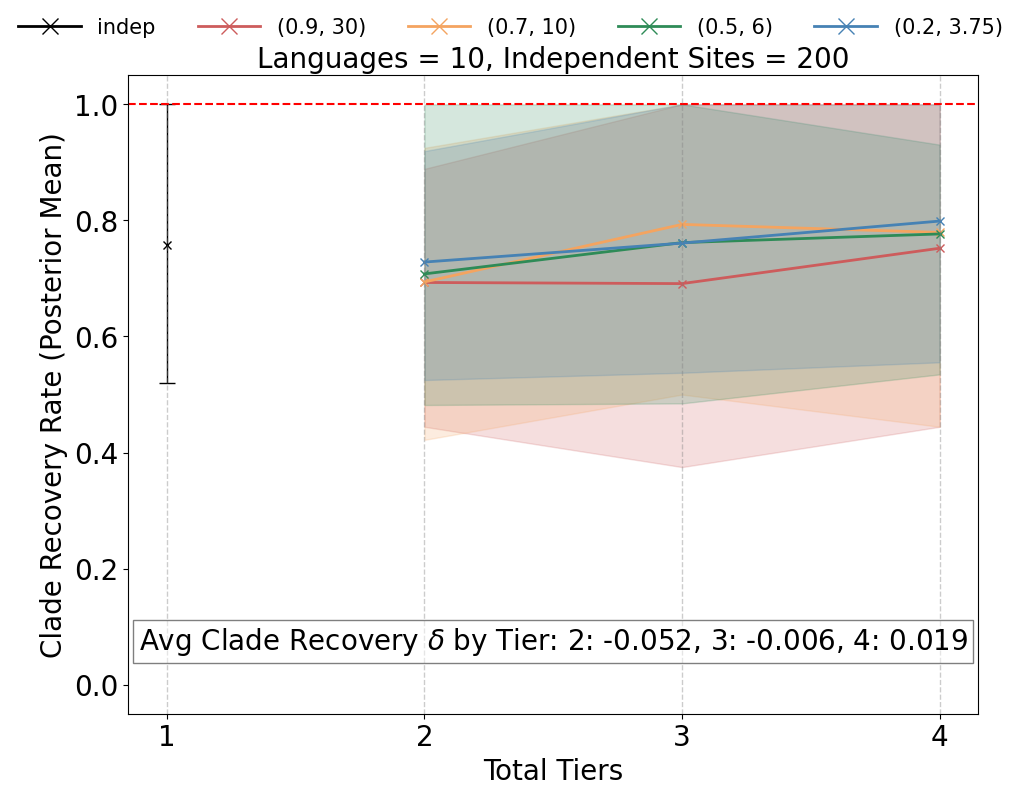
\includegraphics[width=1\linewidth]{figures/exp2highdata.png}
            \end{figure}
        \end{column}
    \end{columns}
\end{frame}

% \begin{frame}
% 	\frametitle{Key Result}
%     Contradiction? Rather... \\
%     \textbf{Effective Information} \\
%     All dependent sites cause model misspecification, but...
%     \vspace{-15mm}
%     \begin{figure}
%         \centering
%         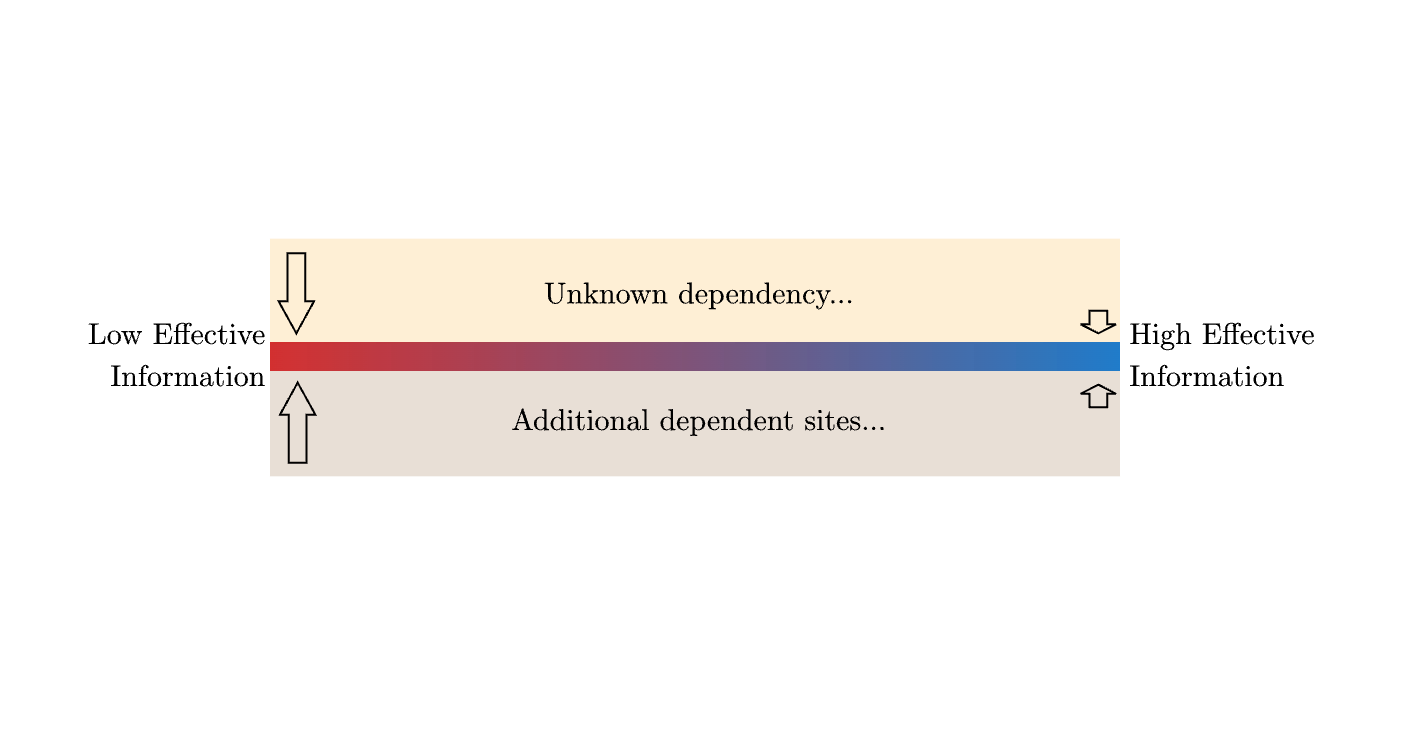
\includegraphics[width=1\linewidth]{figures/image.png}
%         \caption{Caption}
%         \label{fig:placeholder}
%     \end{figure}
% \end{frame}

% \begin{frame}
% 	\frametitle{Conclusion}
%     \textbf{Effective Information vs Model Misspecification} \\
%     Experiment 1: Effects of unknown dependencies \\
%     Experiment 2: Decision-making on retaining dependent sites
% \end{frame}

% \begin{frame}
%     \frametitle{References}
%     \bibliographystyle{abbrvunsrtnat.bst}
%     \bibliography{bibliography}
% \end{frame}


% \begingroup
% 	\setbeamercolor{normal text}{fg=ICLBlue}\usebeamercolor[fg]{normal text} % Slide text color
% 	\setbeamertemplate{closing slide logo}[logo]{ICL_Logo_Blue.pdf} % Imperial logo color, use 'ICL_Logo_White.pdf' for white and 'ICL_Logo_Blue.pdf' for blue
% 	\setbeamertemplate{closing slide text}[text]{Thank you!} % Slide text
	
% 	\usebeamertemplate{closing slide} % Output the closing slide
% \endgroup

%----------------------------------------------------------------------------------------

\end{document}
